\documentclass{jarticle}
\usepackage[dvipdfmx]{graphicx}
\usepackage{here}
\usepackage{listings}

\title{{システム実験}\\基礎実験2}
\author{6119019056 山口力也}
\date{2019/04/日提出}

\begin{document}
\maketitle

\section{概要}
基礎実験第2回目の実験の目的,実施した実験の概要,および理解した事柄を100~200字程度で説明せよ.

本実験では,Arduino開発環境とマイコンのディジタルI/Oを使用した実験を行うことで,Arduinoの基本的な使用方法やマイコンの開発方法を習得した.以下に本実験での目的を示す.

\begin{itemize}

\item Arduino開発環境に慣れる.
\item ArduinoUNOマイコンボードの仕組みを理解する.
\item Arduinoとブレッドボードの接続を行うことができる.
\item ディジタルIOポートの原理を理解する.
\item ディジタルIOポートのプログラムを作成する.

\end{itemize}

\section{マイコンによるLEDの点滅}
演習2.2.1と演習2.2.2のスケッチを報告せよ.また,delay関数の引数を点滅速度との関係について考察せよ.
以下に,演習2.2.1のスケッチを以下に示す.

\begin{lstlisting}
setup() {
  pinMode(13, OUTPUT);//13番ポートを出力に設定
}

void loop() {
  digitalWrite(13, HIGH); //13番ポートにHIGH(5V)を出力 
  delay(500);             //500ms(0.5s)待つ
  digitalWrite(13, LOW);  //13番ポートにLOW(0v)を出力 
  delay(500);             //500ms(0.5s)待つ 
}
\end{lstlisting}

次に演習2.2.2のスケッチを以下に示す.
\begin{lstlisting}

const int LED\_PIN = 13;//13番ポートをLED\_PINとして定義
const int SW\_PIN = 4;//4番ポートをSW\_PINとして定義
int sw1;//swの入力を保存するようの変数を定義
void setup() {
  pinMode(LED\_PIN,OUTPUT);//LED\_PINを出力ポートとして設定
  pinMode(SW\_PIN,INPUT);//SW\_PINを入力ポートとして設定
}

void loop() {
  sw1=digitalRead(SW\_PIN);//sw1にSW\_PINの入力を代入
  if(sw1==LOW){//sw1がLOWのとき(プルアップ抵抗なのでスイッチを押しているとき)
    digitalWrite(LED\_PIN,HIGH);//LED\_PINにHIGH(5V)を出力
  }
  else{//sw1がHIGHのとき(プルアップ抵抗なのでスイッチを押していないとき)
    digitalWrite(LED\_PIN,LOW);//LED\_PINにLOW(0V)を出力
  }
}

\end{lstlisting}

\section{Arduinoによるブレッドボード上のLEDの点滅}
課題2.2.1において実装した回路図,ブレッドボード配線図およびスケッチを報告せよ.また,LEDの動作原理を回路図とあsk受精したプログラムより考察せよ.

課題2.2.1で作成した回路図を以下\ref{fig:2-2-1kairo}に,ブレッドボード配線図を\ref{fig:2-2-1bread}に示す.

\begin{figure}[H]
\begin{center}
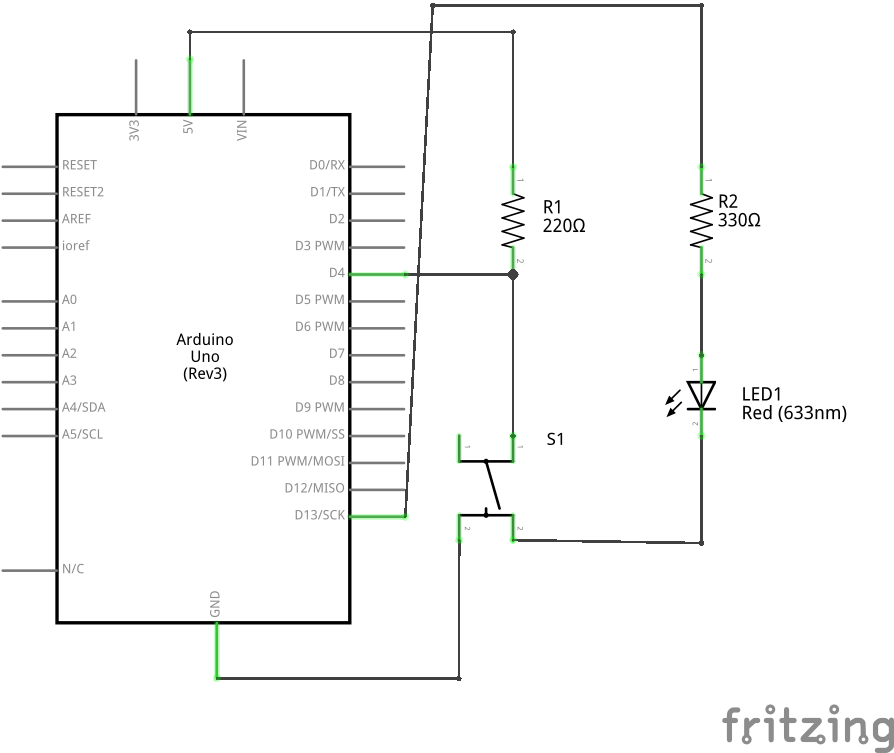
\includegraphics[width=7.0cm]{images/kadai2-2-1_kairo.png}
\caption{課題2.2.1の回路図}
\label{fig:2-2-1kairo}
\end{center}
\end{figure}


\begin{figure}[H]
\begin{center}
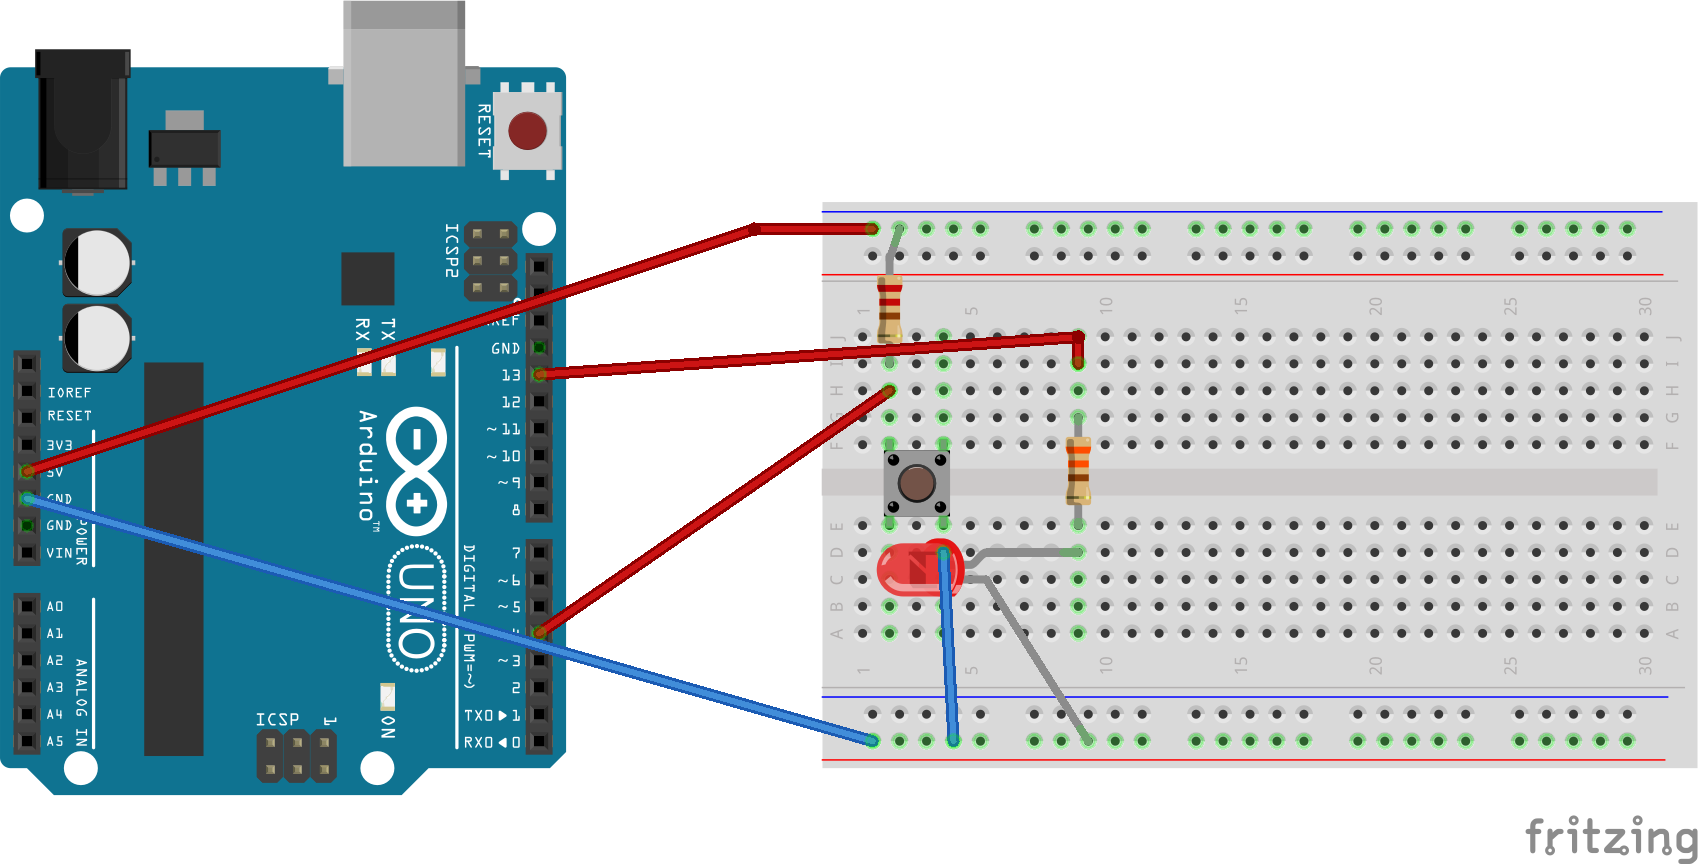
\includegraphics[width=7.0cm]{images/kadai2-2-1_bread.png}
\caption{課題2.2.1の配線図}
\label{fig:2-2-1bread}
\end{center}
\end{figure}


\end{document}
